\section{\bap Overview}

\begin{figure}
\centering
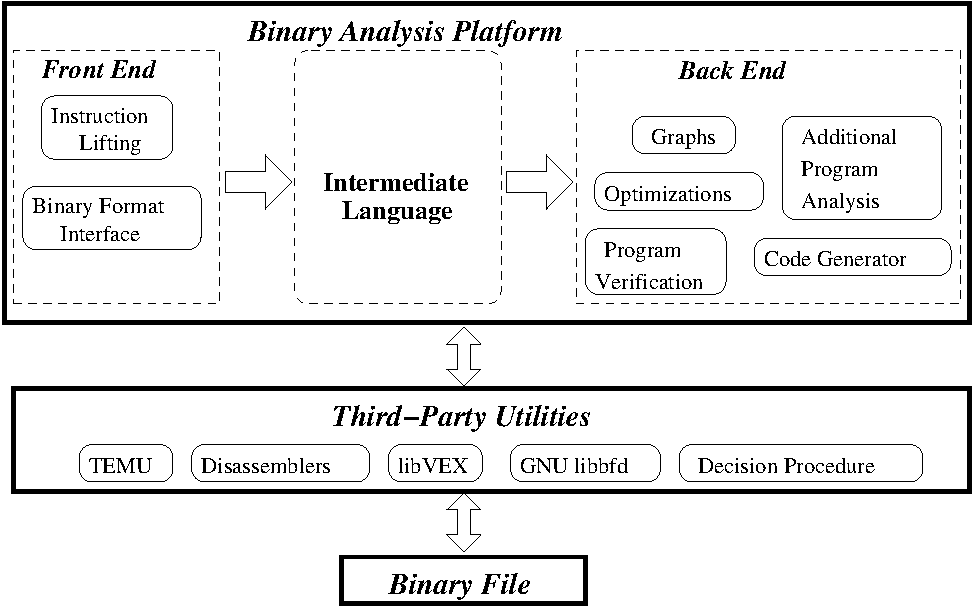
\includegraphics[scale=.8]{fig/components}
\caption{The \bap binary analysis architecture and components. \bap
  is divided into a front-end, which is responsible for lifting
  instructions to the \bap IL, and a platform-independent back-end
  for analyses.}
\label{fig:vine-components}
\end{figure}

\bap  is designed to facilitate faithful
security-relevant binary program analysis by 1) reducing complex
instruction sets to a single, small, and formally specified
intermediate language that supports writing  concise,
easy-to-understand analyses 2) providing a set of core program analyses
abstractions, and 3) being architecture independent when possible in
order to support easy re-targeting.


Figure~\ref{fig:vine-components} shows a high-level picture of \bap.
\bap is divided into an architecture-specific front-end and an
architecture-independent back-end.  At the core of \bap is an
architecture-independent intermediate language (IL), called \emph{\bil,} for
assembly. Assembly instructions in the underlying architecture are
lifted up to the \bil via the \bap front-end.  All analyses are
performed on the platform-independent \bil in the back-end.
%Thus, program analysis can be
%written in an architecture-independent fashion.

We lift to the \bil by using open-source utilities to parse the binary
format and produce assembly.  The assembly is then lifted up to the
\bap IL in a syntax-directed manner. The \bap front-end currently
supports lifting x86~\cite{intel:x86} and ARMv4~\cite{arm:armv4} to
the IL.

The \bap back-end supports a variety of core program analyses
and utilities.  The back-end has utilities for creating a variety of
different graphs, such as control flow and program dependence graphs.
The back-end also provides an optimization framework. The optimization
framework is usually used to simplify a specific set of
instructions. We also provide program verification capabilities such
as symbolic execution, calculating the weakest precondition, and
interfacing with decision procedures.  \bap can also write out lifted
\bap instructions as valid C code via the code generator back-end.


For example, one may want to analyze an execution trace. The execution
trace can be lifted to \bap, then optimized to remove
instructions from the trace that are not relevant to the analysis.
The analysis could then verify properties of the trace by using
program verification routines. Finally, the trace itself could be
written out as a valid C program, compiled down to assembly, and then
run as a straight-line program.


